\documentclass[1p]{elsarticle_modified}
%\bibliographystyle{elsarticle-num}

%\usepackage[colorlinks]{hyperref}
%\usepackage{abbrmath_seonhwa} %\Abb, \Ascr, \Acal ,\Abf, \Afrak
\usepackage{amsfonts}
\usepackage{amssymb}
\usepackage{amsmath}
\usepackage{amsthm}
\usepackage{scalefnt}
\usepackage{amsbsy}
\usepackage{kotex}
\usepackage{caption}
\usepackage{subfig}
\usepackage{color}
\usepackage{graphicx}
\usepackage{xcolor} %% white, black, red, green, blue, cyan, magenta, yellow
\usepackage{float}
\usepackage{setspace}
\usepackage{hyperref}

\usepackage{tikz}
\usetikzlibrary{arrows}

\usepackage{multirow}
\usepackage{array} % fixed length table
\usepackage{hhline}

%%%%%%%%%%%%%%%%%%%%%
\makeatletter
\renewcommand*\env@matrix[1][\arraystretch]{%
	\edef\arraystretch{#1}%
	\hskip -\arraycolsep
	\let\@ifnextchar\new@ifnextchar
	\array{*\c@MaxMatrixCols c}}
\makeatother %https://tex.stackexchange.com/questions/14071/how-can-i-increase-the-line-spacing-in-a-matrix
%%%%%%%%%%%%%%%

\usepackage[normalem]{ulem}

\newcommand{\msout}[1]{\ifmmode\text{\sout{\ensuremath{#1}}}\else\sout{#1}\fi}
%SOURCE: \msout is \stkout macro in https://tex.stackexchange.com/questions/20609/strikeout-in-math-mode

\newcommand{\cancel}[1]{
	\ifmmode
	{\color{red}\msout{#1}}
	\else
	{\color{red}\sout{#1}}
	\fi
}

\newcommand{\add}[1]{
	{\color{blue}\uwave{#1}}
}

\newcommand{\replace}[2]{
	\ifmmode
	{\color{red}\msout{#1}}{\color{blue}\uwave{#2}}
	\else
	{\color{red}\sout{#1}}{\color{blue}\uwave{#2}}
	\fi
}

\newcommand{\Sol}{\mathcal{S}} %segment
\newcommand{\D}{D} %diagram
\newcommand{\A}{\mathcal{A}} %arc


%%%%%%%%%%%%%%%%%%%%%%%%%%%%%5 test

\def\sl{\operatorname{\textup{SL}}(2,\Cbb)}
\def\psl{\operatorname{\textup{PSL}}(2,\Cbb)}
\def\quan{\mkern 1mu \triangleright \mkern 1mu}

\theoremstyle{definition}
\newtheorem{thm}{Theorem}[section]
\newtheorem{prop}[thm]{Proposition}
\newtheorem{lem}[thm]{Lemma}
\newtheorem{ques}[thm]{Question}
\newtheorem{cor}[thm]{Corollary}
\newtheorem{defn}[thm]{Definition}
\newtheorem{exam}[thm]{Example}
\newtheorem{rmk}[thm]{Remark}
\newtheorem{alg}[thm]{Algorithm}

\newcommand{\I}{\sqrt{-1}}
\begin{document}

%\begin{frontmatter}
%
%\title{Boundary parabolic representations of knots up to 8 crossings}
%
%%% Group authors per affiliation:
%\author{Yunhi Cho} 
%\address{Department of Mathematics, University of Seoul, Seoul, Korea}
%\ead{yhcho@uos.ac.kr}
%
%
%\author{Seonhwa Kim} %\fnref{s_kim}}
%\address{Center for Geometry and Physics, Institute for Basic Science, Pohang, 37673, Korea}
%\ead{ryeona17@ibs.re.kr}
%
%\author{Hyuk Kim}
%\address{Department of Mathematical Sciences, Seoul National University, Seoul 08826, Korea}
%\ead{hyukkim@snu.ac.kr}
%
%\author{Seokbeom Yoon}
%\address{Department of Mathematical Sciences, Seoul National University, Seoul, 08826,  Korea}
%\ead{sbyoon15@snu.ac.kr}
%
%\begin{abstract}
%We find all boundary parabolic representation of knots up to 8 crossings.
%
%\end{abstract}
%\begin{keyword}
%    \MSC[2010] 57M25 
%\end{keyword}
%
%\end{frontmatter}

%\linenumbers
%\tableofcontents
%
\newcommand\colored[1]{\textcolor{white}{\rule[-0.35ex]{0.8em}{1.4ex}}\kern-0.8em\color{red} #1}%
%\newcommand\colored[1]{\textcolor{white}{ #1}\kern-2.17ex	\textcolor{white}{ #1}\kern-1.81ex	\textcolor{white}{ #1}\kern-2.15ex\color{red}#1	}

{\Large $\underline{12n_{0499}~(K12n_{0499})}$}

\setlength{\tabcolsep}{10pt}
\renewcommand{\arraystretch}{1.6}
\vspace{1cm}\begin{tabular}{m{100pt}>{\centering\arraybackslash}m{274pt}}
\multirow{5}{120pt}{
	\centering
	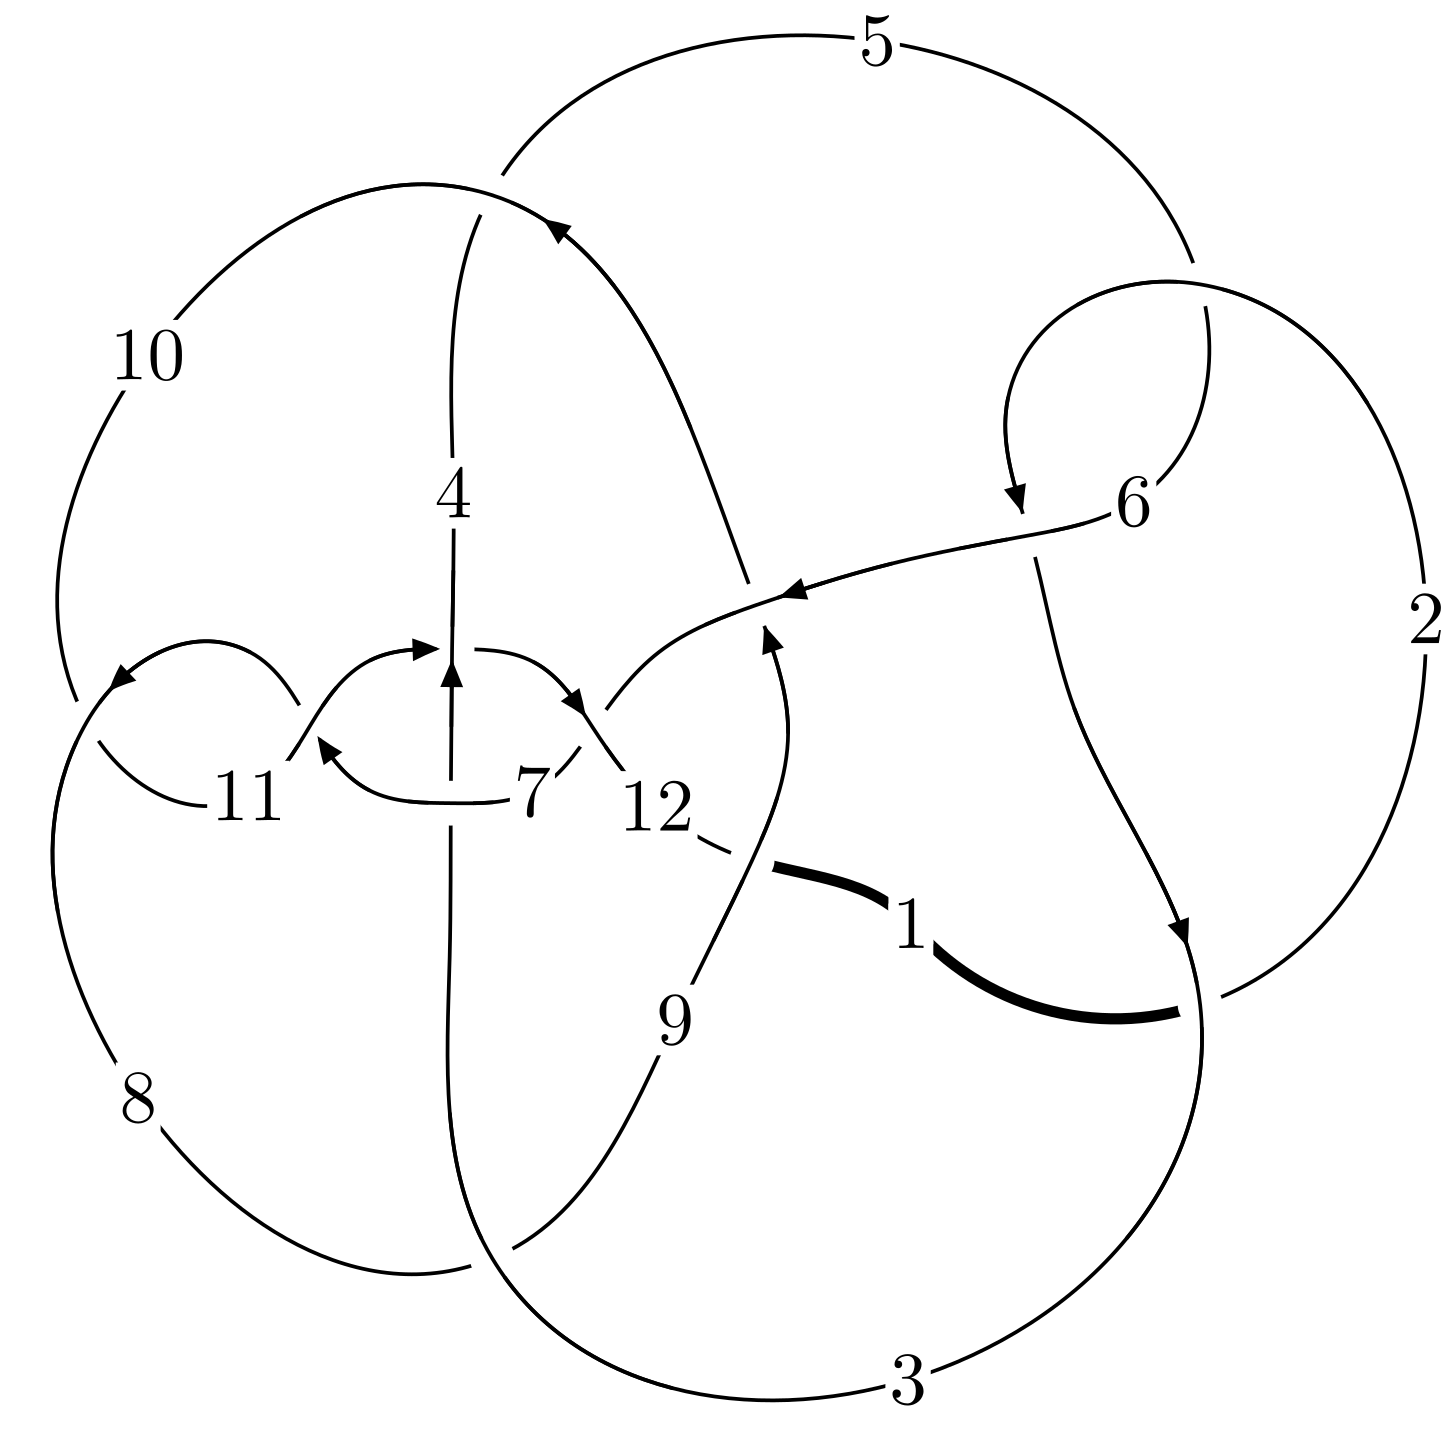
\includegraphics[width=112pt]{../../../GIT/diagram.site/Diagrams/png/2588_12n_0499.png}\\
\ \ \ A knot diagram\footnotemark}&
\allowdisplaybreaks
\textbf{Linearized knot diagam} \\
\cline{2-2}
 &
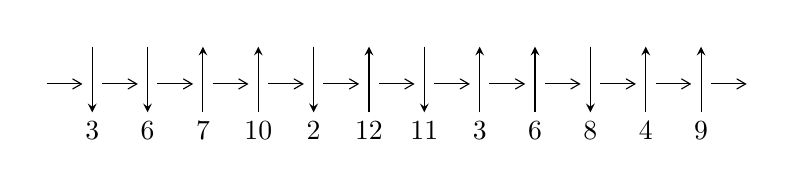
\begin{tikzpicture}[x=20pt, y=17pt]
	% nodes
	\node (C0) at (0, 0) {};
	\node (C1) at (1, 0) {};
	\node (C1U) at (1, +1) {};
	\node (C1D) at (1, -1) {3};

	\node (C2) at (2, 0) {};
	\node (C2U) at (2, +1) {};
	\node (C2D) at (2, -1) {6};

	\node (C3) at (3, 0) {};
	\node (C3U) at (3, +1) {};
	\node (C3D) at (3, -1) {7};

	\node (C4) at (4, 0) {};
	\node (C4U) at (4, +1) {};
	\node (C4D) at (4, -1) {10};

	\node (C5) at (5, 0) {};
	\node (C5U) at (5, +1) {};
	\node (C5D) at (5, -1) {2};

	\node (C6) at (6, 0) {};
	\node (C6U) at (6, +1) {};
	\node (C6D) at (6, -1) {12};

	\node (C7) at (7, 0) {};
	\node (C7U) at (7, +1) {};
	\node (C7D) at (7, -1) {11};

	\node (C8) at (8, 0) {};
	\node (C8U) at (8, +1) {};
	\node (C8D) at (8, -1) {3};

	\node (C9) at (9, 0) {};
	\node (C9U) at (9, +1) {};
	\node (C9D) at (9, -1) {6};

	\node (C10) at (10, 0) {};
	\node (C10U) at (10, +1) {};
	\node (C10D) at (10, -1) {8};

	\node (C11) at (11, 0) {};
	\node (C11U) at (11, +1) {};
	\node (C11D) at (11, -1) {4};

	\node (C12) at (12, 0) {};
	\node (C12U) at (12, +1) {};
	\node (C12D) at (12, -1) {9};
	\node (C13) at (13, 0) {};

	% arrows
	\draw[->,>={angle 60}]
	(C0) edge (C1) (C1) edge (C2) (C2) edge (C3) (C3) edge (C4) (C4) edge (C5) (C5) edge (C6) (C6) edge (C7) (C7) edge (C8) (C8) edge (C9) (C9) edge (C10) (C10) edge (C11) (C11) edge (C12) (C12) edge (C13) ;	\draw[->,>=stealth]
	(C1U) edge (C1D) (C2U) edge (C2D) (C3D) edge (C3U) (C4D) edge (C4U) (C5U) edge (C5D) (C6D) edge (C6U) (C7U) edge (C7D) (C8D) edge (C8U) (C9D) edge (C9U) (C10U) edge (C10D) (C11D) edge (C11U) (C12D) edge (C12U) ;
	\end{tikzpicture} \\
\hhline{~~} \\& 
\textbf{Solving Sequence} \\ \cline{2-2} 
 &
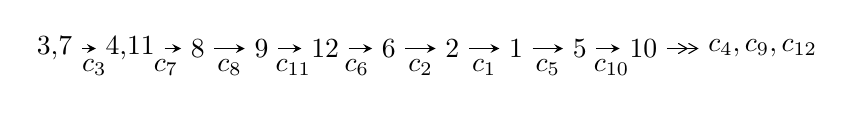
\begin{tikzpicture}[x=23pt, y=7pt]
	% node
	\node (A0) at (-1/8, 0) {3,7};
	\node (A1) at (17/16, 0) {4,11};
	\node (A2) at (17/8, 0) {8};
	\node (A3) at (25/8, 0) {9};
	\node (A4) at (33/8, 0) {12};
	\node (A5) at (41/8, 0) {6};
	\node (A6) at (49/8, 0) {2};
	\node (A7) at (57/8, 0) {1};
	\node (A8) at (65/8, 0) {5};
	\node (A9) at (73/8, 0) {10};
	\node (C1) at (1/2, -1) {$c_{3}$};
	\node (C2) at (13/8, -1) {$c_{7}$};
	\node (C3) at (21/8, -1) {$c_{8}$};
	\node (C4) at (29/8, -1) {$c_{11}$};
	\node (C5) at (37/8, -1) {$c_{6}$};
	\node (C6) at (45/8, -1) {$c_{2}$};
	\node (C7) at (53/8, -1) {$c_{1}$};
	\node (C8) at (61/8, -1) {$c_{5}$};
	\node (C9) at (69/8, -1) {$c_{10}$};
	\node (A10) at (11, 0) {$c_{4},c_{9},c_{12}$};

	% edge
	\draw[->,>=stealth]	
	(A0) edge (A1) (A1) edge (A2) (A2) edge (A3) (A3) edge (A4) (A4) edge (A5) (A5) edge (A6) (A6) edge (A7) (A7) edge (A8) (A8) edge (A9) ;
	\draw[->>,>={angle 60}]	
	(A9) edge (A10);
\end{tikzpicture} \\ 

\end{tabular} \\

\footnotetext{
The image of knot diagram is generated by the software ``\textbf{Draw programme}" developed by Andrew Bartholomew(\url{http://www.layer8.co.uk/maths/draw/index.htm\#Running-draw}), where we modified some parts for our purpose(\url{https://github.com/CATsTAILs/LinksPainter}).
}\phantom \\ \newline 
\centering \textbf{Ideals for irreducible components\footnotemark of $X_{\text{par}}$} 
 
\begin{align*}
I^u_{1}&=\langle 
253607 u^{17}-119815 u^{16}+\cdots+2792 b+534547,\\
\phantom{I^u_{1}}&\phantom{= \langle  }-1130011 u^{17}+534547 u^{16}+\cdots+2792 a-2385431,\\
\phantom{I^u_{1}}&\phantom{= \langle  }u^{18}- u^{16}+u^{15}+9 u^{14}+u^{13}-6 u^{12}+3 u^{11}+21 u^{10}+4 u^9-7 u^8+5 u^7+16 u^6-9 u^4-9 u^3- u^2+3 u+1\rangle \\
I^u_{2}&=\langle 
u^{11}+u^{10}-3 u^9+2 u^8+7 u^7-6 u^5+6 u^4+8 u^3-8 u^2+4 b+u+3,\\
\phantom{I^u_{2}}&\phantom{= \langle  }-9 u^{11}+3 u^{10}- u^9-10 u^8-39 u^7+4 u^6-22 u^5-30 u^4-36 u^3+12 u^2+4 a-17 u-7,\\
\phantom{I^u_{2}}&\phantom{= \langle  }u^{12}+u^9+5 u^8+u^7+2 u^6+4 u^5+6 u^4+u^2+2 u+1\rangle \\
I^u_{3}&=\langle 
4.82591\times10^{21} u^{23}-1.43753\times10^{22} u^{22}+\cdots+2.64783\times10^{21} b+1.78802\times10^{22},\\
\phantom{I^u_{3}}&\phantom{= \langle  }9.78596\times10^{19} u^{23}-3.52311\times10^{20} u^{22}+\cdots+1.93272\times10^{19} a+1.09980\times10^{20},\;u^{24}-3 u^{23}+\cdots+8 u+1\rangle \\
I^u_{4}&=\langle 
5 u^7-18 u^6+14 u^5-17 u^4+44 u^3-53 u^2+11 b+21,\\
\phantom{I^u_{4}}&\phantom{= \langle  }-7 u^7+23 u^6-24 u^5+26 u^4-66 u^3+83 u^2+11 a-22 u-14,\\
\phantom{I^u_{4}}&\phantom{= \langle  }u^8-2 u^7+u^6-2 u^5+6 u^4-4 u^3-2 u^2+2 u+1\rangle \\
\\
\end{align*}
\raggedright * 4 irreducible components of $\dim_{\mathbb{C}}=0$, with total 62 representations.\\
\footnotetext{All coefficients of polynomials are rational numbers. But the coefficients are sometimes approximated in decimal forms when there is not enough margin.}
\newpage
\renewcommand{\arraystretch}{1}
\centering \section*{I. $I^u_{1}= \langle 253607 u^{17}-119815 u^{16}+\cdots+2792 b+534547,\;-1.13\times10^{6} u^{17}+5.35\times10^{5} u^{16}+\cdots+2792 a-2.39\times10^{6},\;u^{18}- u^{16}+\cdots+3 u+1 \rangle$}
\flushleft \textbf{(i) Arc colorings}\\
\begin{tabular}{m{7pt} m{180pt} m{7pt} m{180pt} }
\flushright $a_{3}=$&$\begin{pmatrix}1\\0\end{pmatrix}$ \\
\flushright $a_{7}=$&$\begin{pmatrix}0\\u\end{pmatrix}$ \\
\flushright $a_{4}=$&$\begin{pmatrix}1\\- u^2\end{pmatrix}$ \\
\flushright $a_{11}=$&$\begin{pmatrix}404.732 u^{17}-191.457 u^{16}+\cdots+757.847 u+854.381\\-90.8335 u^{17}+42.9137 u^{16}+\cdots-168.638 u-191.457\end{pmatrix}$ \\
\flushright $a_{8}=$&$\begin{pmatrix}-123.317 u^{17}+57.5845 u^{16}+\cdots-226.145 u-262.067\\-63.4466 u^{17}+30.0842 u^{16}+\cdots-119.201 u-133.872\end{pmatrix}$ \\
\flushright $a_{9}=$&$\begin{pmatrix}-186.763 u^{17}+87.6687 u^{16}+\cdots-345.346 u-395.939\\-63.4466 u^{17}+30.0842 u^{16}+\cdots-119.201 u-133.872\end{pmatrix}$ \\
\flushright $a_{12}=$&$\begin{pmatrix}404.732 u^{17}-191.457 u^{16}+\cdots+758.847 u+854.381\\-90.8335 u^{17}+42.9137 u^{16}+\cdots-168.638 u-191.457\end{pmatrix}$ \\
\flushright $a_{6}=$&$\begin{pmatrix}-304.984 u^{17}+143.412 u^{16}+\cdots-565.421 u-644.981\\-22.6307 u^{17}+10.9817 u^{16}+\cdots-43.3861 u-48.0448\end{pmatrix}$ \\
\flushright $a_{2}=$&$\begin{pmatrix}94.9466 u^{17}-43.5842 u^{16}+\cdots+171.201 u+201.372\\28.6734 u^{17}-13.9162 u^{16}+\cdots+55.9921 u+60.8231\end{pmatrix}$ \\
\flushright $a_{1}=$&$\begin{pmatrix}123.620 u^{17}-57.5004 u^{16}+\cdots+227.193 u+262.195\\28.6734 u^{17}-13.9162 u^{16}+\cdots+55.9921 u+60.8231\end{pmatrix}$ \\
\flushright $a_{5}=$&$\begin{pmatrix}-335.524 u^{17}+158.659 u^{16}+\cdots-631.124 u-712.169\\2.32450 u^{17}-0.887536 u^{16}+\cdots+5.26934 u+6.20702\end{pmatrix}$ \\
\flushright $a_{10}=$&$\begin{pmatrix}-406.592 u^{17}+193.199 u^{16}+\cdots-766.342 u-859.336\\27.5838 u^{17}-13.1547 u^{16}+\cdots+53.8030 u+59.3266\end{pmatrix}$\\&\end{tabular}
\flushleft \textbf{(ii) Obstruction class $= -1$}\\~\\
\flushleft \textbf{(iii) Cusp Shapes $= \frac{2045515}{2792} u^{17}-\frac{964335}{2792} u^{16}+\cdots+\frac{1913265}{1396} u+\frac{4343639}{2792}$}\\~\\
\newpage\renewcommand{\arraystretch}{1}
\flushleft \textbf{(iv) u-Polynomials at the component}\newline \\
\begin{tabular}{m{50pt}|m{274pt}}
Crossings & \hspace{64pt}u-Polynomials at each crossing \\
\hline $$\begin{aligned}c_{1}\end{aligned}$$&$\begin{aligned}
&u^{18}+38 u^{17}+\cdots+21004 u+2704
\end{aligned}$\\
\hline $$\begin{aligned}c_{2},c_{5}\end{aligned}$$&$\begin{aligned}
&u^{18}+12 u^{17}+\cdots-42 u+52
\end{aligned}$\\
\hline $$\begin{aligned}c_{3},c_{11}\end{aligned}$$&$\begin{aligned}
&u^{18}- u^{16}+\cdots+3 u+1
\end{aligned}$\\
\hline $$\begin{aligned}c_{4},c_{8}\end{aligned}$$&$\begin{aligned}
&u^{18}- u^{17}+\cdots-6 u^2+1
\end{aligned}$\\
\hline $$\begin{aligned}c_{6}\end{aligned}$$&$\begin{aligned}
&u^{18}-13 u^{17}+\cdots-184 u+32
\end{aligned}$\\
\hline $$\begin{aligned}c_{7},c_{10}\end{aligned}$$&$\begin{aligned}
&u^{18}-11 u^{17}+\cdots-34 u+4
\end{aligned}$\\
\hline $$\begin{aligned}c_{9},c_{12}\end{aligned}$$&$\begin{aligned}
&u^{18}+u^{17}+\cdots+27 u+2
\end{aligned}$\\
\hline
\end{tabular}\\~\\
\newpage\renewcommand{\arraystretch}{1}
\flushleft \textbf{(v) Riley Polynomials at the component}\newline \\
\begin{tabular}{m{50pt}|m{274pt}}
Crossings & \hspace{64pt}Riley Polynomials at each crossing \\
\hline $$\begin{aligned}c_{1}\end{aligned}$$&$\begin{aligned}
&y^{18}-146 y^{17}+\cdots-126806384 y+7311616
\end{aligned}$\\
\hline $$\begin{aligned}c_{2},c_{5}\end{aligned}$$&$\begin{aligned}
&y^{18}-38 y^{17}+\cdots-21004 y+2704
\end{aligned}$\\
\hline $$\begin{aligned}c_{3},c_{11}\end{aligned}$$&$\begin{aligned}
&y^{18}-2 y^{17}+\cdots-11 y+1
\end{aligned}$\\
\hline $$\begin{aligned}c_{4},c_{8}\end{aligned}$$&$\begin{aligned}
&y^{18}+29 y^{17}+\cdots-12 y+1
\end{aligned}$\\
\hline $$\begin{aligned}c_{6}\end{aligned}$$&$\begin{aligned}
&y^{18}+3 y^{17}+\cdots+8896 y+1024
\end{aligned}$\\
\hline $$\begin{aligned}c_{7},c_{10}\end{aligned}$$&$\begin{aligned}
&y^{18}+7 y^{17}+\cdots+212 y+16
\end{aligned}$\\
\hline $$\begin{aligned}c_{9},c_{12}\end{aligned}$$&$\begin{aligned}
&y^{18}+41 y^{17}+\cdots-53 y+4
\end{aligned}$\\
\hline
\end{tabular}\\~\\
\newpage\flushleft \textbf{(vi) Complex Volumes and Cusp Shapes}
$$\begin{array}{c|c|c}  
\text{Solutions to }I^u_{1}& \I (\text{vol} + \sqrt{-1}CS) & \text{Cusp shape}\\
 \hline 
\begin{aligned}
u &= -0.891966 + 0.505299 I \\
a &= -0.23675 - 1.79433 I \\
b &= \phantom{-}0.85339 + 1.26132 I\end{aligned}
 & -12.21600 - 5.30943 I & \phantom{-}1.96728 + 5.12021 I \\ \hline\begin{aligned}
u &= -0.891966 - 0.505299 I \\
a &= -0.23675 + 1.79433 I \\
b &= \phantom{-}0.85339 - 1.26132 I\end{aligned}
 & -12.21600 + 5.30943 I & \phantom{-}1.96728 - 5.12021 I \\ \hline\begin{aligned}
u &= \phantom{-}0.578165 + 0.938615 I \\
a &= \phantom{-}1.09411 - 1.04806 I \\
b &= \phantom{-}0.038828 - 0.821875 I\end{aligned}
 & -18.0039 + 5.4690 I & -2.64879 - 4.54026 I \\ \hline\begin{aligned}
u &= \phantom{-}0.578165 - 0.938615 I \\
a &= \phantom{-}1.09411 + 1.04806 I \\
b &= \phantom{-}0.038828 + 0.821875 I\end{aligned}
 & -18.0039 - 5.4690 I & -2.64879 + 4.54026 I \\ \hline\begin{aligned}
u &= -0.854287 + 0.898221 I \\
a &= \phantom{-}0.539073 - 0.616267 I \\
b &= \phantom{-}0.13299 + 1.67807 I\end{aligned}
 & -0.401628 - 0.023944 I & \phantom{-}0.798667 - 0.224914 I \\ \hline\begin{aligned}
u &= -0.854287 - 0.898221 I \\
a &= \phantom{-}0.539073 + 0.616267 I \\
b &= \phantom{-}0.13299 - 1.67807 I\end{aligned}
 & -0.401628 + 0.023944 I & \phantom{-}0.798667 + 0.224914 I \\ \hline\begin{aligned}
u &= -0.241248 + 0.688870 I \\
a &= -0.525924 + 0.059772 I \\
b &= -0.480079 + 0.538950 I\end{aligned}
 & -1.87297 + 1.40233 I & -2.30233 - 2.52603 I \\ \hline\begin{aligned}
u &= -0.241248 - 0.688870 I \\
a &= -0.525924 - 0.059772 I \\
b &= -0.480079 - 0.538950 I\end{aligned}
 & -1.87297 - 1.40233 I & -2.30233 + 2.52603 I \\ \hline\begin{aligned}
u &= \phantom{-}1.069570 + 0.765142 I \\
a &= -0.272123 - 0.684036 I \\
b &= \phantom{-}0.10197 + 1.59259 I\end{aligned}
 & \phantom{-}2.96611 + 2.61050 I & \phantom{-}7.54398 - 1.84581 I \\ \hline\begin{aligned}
u &= \phantom{-}1.069570 - 0.765142 I \\
a &= -0.272123 + 0.684036 I \\
b &= \phantom{-}0.10197 - 1.59259 I\end{aligned}
 & \phantom{-}2.96611 - 2.61050 I & \phantom{-}7.54398 + 1.84581 I\\
 \hline 
 \end{array}$$\newpage$$\begin{array}{c|c|c}  
\text{Solutions to }I^u_{1}& \I (\text{vol} + \sqrt{-1}CS) & \text{Cusp shape}\\
 \hline 
\begin{aligned}
u &= \phantom{-}0.678153 + 0.019544 I \\
a &= \phantom{-}0.966784 + 0.264491 I \\
b &= \phantom{-}0.240917 - 0.127619 I\end{aligned}
 & \phantom{-}1.208600 + 0.022955 I & \phantom{-}9.69868 + 0.48984 I \\ \hline\begin{aligned}
u &= \phantom{-}0.678153 - 0.019544 I \\
a &= \phantom{-}0.966784 - 0.264491 I \\
b &= \phantom{-}0.240917 + 0.127619 I\end{aligned}
 & \phantom{-}1.208600 - 0.022955 I & \phantom{-}9.69868 - 0.48984 I \\ \hline\begin{aligned}
u &= -1.043070 + 0.939013 I \\
a &= -0.010456 - 0.755078 I \\
b &= \phantom{-}0.438217 + 1.074260 I\end{aligned}
 & -0.86599 - 7.63655 I & \phantom{-}0.42339 + 4.89613 I \\ \hline\begin{aligned}
u &= -1.043070 - 0.939013 I \\
a &= -0.010456 + 0.755078 I \\
b &= \phantom{-}0.438217 - 1.074260 I\end{aligned}
 & -0.86599 + 7.63655 I & \phantom{-}0.42339 - 4.89613 I \\ \hline\begin{aligned}
u &= -0.473262 + 0.000907 I \\
a &= -0.32200 + 3.04257 I \\
b &= -0.403752 - 0.680833 I\end{aligned}
 & \phantom{-}1.20753 - 2.46681 I & \phantom{-}11.74185 + 5.49254 I \\ \hline\begin{aligned}
u &= -0.473262 - 0.000907 I \\
a &= -0.32200 - 3.04257 I \\
b &= -0.403752 + 0.680833 I\end{aligned}
 & \phantom{-}1.20753 + 2.46681 I & \phantom{-}11.74185 - 5.49254 I \\ \hline\begin{aligned}
u &= \phantom{-}1.17795 + 1.15587 I \\
a &= -0.232707 - 0.959348 I \\
b &= -1.42248 + 1.83898 I\end{aligned}
 & -14.7900 + 13.6947 I & -0.22273 - 6.15238 I \\ \hline\begin{aligned}
u &= \phantom{-}1.17795 - 1.15587 I \\
a &= -0.232707 + 0.959348 I \\
b &= -1.42248 - 1.83898 I\end{aligned}
 & -14.7900 - 13.6947 I & -0.22273 + 6.15238 I\\
 \hline 
 \end{array}$$\newpage\newpage\renewcommand{\arraystretch}{1}
\centering \section*{II. $I^u_{2}= \langle u^{11}+u^{10}+\cdots+4 b+3,\;-9 u^{11}+3 u^{10}+\cdots+4 a-7,\;u^{12}+u^9+\cdots+2 u+1 \rangle$}
\flushleft \textbf{(i) Arc colorings}\\
\begin{tabular}{m{7pt} m{180pt} m{7pt} m{180pt} }
\flushright $a_{3}=$&$\begin{pmatrix}1\\0\end{pmatrix}$ \\
\flushright $a_{7}=$&$\begin{pmatrix}0\\u\end{pmatrix}$ \\
\flushright $a_{4}=$&$\begin{pmatrix}1\\- u^2\end{pmatrix}$ \\
\flushright $a_{11}=$&$\begin{pmatrix}\frac{9}{4} u^{11}-\frac{3}{4} u^{10}+\cdots+\frac{17}{4} u+\frac{7}{4}\\-\frac{1}{4} u^{11}-\frac{1}{4} u^{10}+\cdots-\frac{1}{4} u-\frac{3}{4}\end{pmatrix}$ \\
\flushright $a_{8}=$&$\begin{pmatrix}\frac{1}{2} u^{11}- u^{10}+\cdots+\frac{5}{2} u-4\\-\frac{5}{4} u^{11}+\frac{5}{4} u^{10}+\cdots-\frac{5}{4} u-\frac{1}{4}\end{pmatrix}$ \\
\flushright $a_{9}=$&$\begin{pmatrix}-\frac{3}{4} u^{11}+\frac{1}{4} u^{10}+\cdots+\frac{5}{4} u-\frac{17}{4}\\-\frac{5}{4} u^{11}+\frac{5}{4} u^{10}+\cdots-\frac{5}{4} u-\frac{1}{4}\end{pmatrix}$ \\
\flushright $a_{12}=$&$\begin{pmatrix}\frac{9}{4} u^{11}-\frac{3}{4} u^{10}+\cdots+\frac{13}{4} u+\frac{7}{4}\\-\frac{1}{4} u^{11}-\frac{1}{4} u^{10}+\cdots-\frac{1}{4} u-\frac{3}{4}\end{pmatrix}$ \\
\flushright $a_{6}=$&$\begin{pmatrix}u^{11}-\frac{1}{2} u^{10}+\cdots+u-\frac{5}{2}\\\frac{1}{4} u^{11}+\frac{3}{4} u^{10}+\cdots+\frac{1}{4} u+\frac{1}{4}\end{pmatrix}$ \\
\flushright $a_{2}=$&$\begin{pmatrix}-\frac{3}{4} u^{11}+\frac{7}{4} u^{10}+\cdots-\frac{15}{4} u-\frac{7}{4}\\\frac{1}{4} u^{11}+\frac{5}{4} u^{10}+\cdots+\frac{9}{4} u+\frac{7}{4}\end{pmatrix}$ \\
\flushright $a_{1}=$&$\begin{pmatrix}-\frac{1}{2} u^{11}+3 u^{10}+\cdots+5 u^2-\frac{3}{2} u\\\frac{1}{4} u^{11}+\frac{5}{4} u^{10}+\cdots+\frac{9}{4} u+\frac{7}{4}\end{pmatrix}$ \\
\flushright $a_{5}=$&$\begin{pmatrix}\frac{3}{4} u^{11}-\frac{7}{4} u^{10}+\cdots+\frac{3}{4} u-\frac{13}{4}\\\frac{1}{2} u^{11}-2 u^{10}+\cdots-\frac{5}{2} u-2\end{pmatrix}$ \\
\flushright $a_{10}=$&$\begin{pmatrix}-\frac{5}{2} u^{11}+\frac{3}{2} u^{10}+\cdots-\frac{9}{2} u-\frac{17}{2}\\\frac{3}{4} u^{11}+\frac{1}{4} u^{10}+\cdots+\frac{7}{4} u+\frac{7}{4}\end{pmatrix}$\\&\end{tabular}
\flushleft \textbf{(ii) Obstruction class $= 1$}\\~\\
\flushleft \textbf{(iii) Cusp Shapes $= \frac{43}{4} u^{11}-\frac{23}{4} u^{10}-\frac{5}{4} u^9+13 u^8+\frac{183}{4} u^7-17 u^6+\frac{25}{2} u^5+\frac{69}{2} u^4+36 u^3-30 u^2+\frac{35}{4} u+\frac{63}{4}$}\\~\\
\newpage\renewcommand{\arraystretch}{1}
\flushleft \textbf{(iv) u-Polynomials at the component}\newline \\
\begin{tabular}{m{50pt}|m{274pt}}
Crossings & \hspace{64pt}u-Polynomials at each crossing \\
\hline $$\begin{aligned}c_{1}\end{aligned}$$&$\begin{aligned}
&u^{12}-11 u^{11}+\cdots+38 u+9
\end{aligned}$\\
\hline $$\begin{aligned}c_{2}\end{aligned}$$&$\begin{aligned}
&u^{12}+7 u^{11}+\cdots+8 u+3
\end{aligned}$\\
\hline $$\begin{aligned}c_{3},c_{11}\end{aligned}$$&$\begin{aligned}
&u^{12}+u^9+5 u^8+u^7+2 u^6+4 u^5+6 u^4+u^2+2 u+1
\end{aligned}$\\
\hline $$\begin{aligned}c_{4},c_{8}\end{aligned}$$&$\begin{aligned}
&u^{12}+u^{11}+\cdots+3 u+1
\end{aligned}$\\
\hline $$\begin{aligned}c_{5}\end{aligned}$$&$\begin{aligned}
&u^{12}-7 u^{11}+\cdots-8 u+3
\end{aligned}$\\
\hline $$\begin{aligned}c_{6}\end{aligned}$$&$\begin{aligned}
&u^{12}-6 u^{11}+\cdots-2 u+1
\end{aligned}$\\
\hline $$\begin{aligned}c_{7}\end{aligned}$$&$\begin{aligned}
&u^{12}-6 u^{11}+\cdots-26 u+7
\end{aligned}$\\
\hline $$\begin{aligned}c_{9},c_{12}\end{aligned}$$&$\begin{aligned}
&u^{12}- u^{11}+\cdots-3 u+1
\end{aligned}$\\
\hline $$\begin{aligned}c_{10}\end{aligned}$$&$\begin{aligned}
&u^{12}+6 u^{11}+\cdots+26 u+7
\end{aligned}$\\
\hline
\end{tabular}\\~\\
\newpage\renewcommand{\arraystretch}{1}
\flushleft \textbf{(v) Riley Polynomials at the component}\newline \\
\begin{tabular}{m{50pt}|m{274pt}}
Crossings & \hspace{64pt}Riley Polynomials at each crossing \\
\hline $$\begin{aligned}c_{1}\end{aligned}$$&$\begin{aligned}
&y^{12}-31 y^{11}+\cdots-814 y+81
\end{aligned}$\\
\hline $$\begin{aligned}c_{2},c_{5}\end{aligned}$$&$\begin{aligned}
&y^{12}-11 y^{11}+\cdots+38 y+9
\end{aligned}$\\
\hline $$\begin{aligned}c_{3},c_{11}\end{aligned}$$&$\begin{aligned}
&y^{12}+10 y^{10}+\cdots-2 y+1
\end{aligned}$\\
\hline $$\begin{aligned}c_{4},c_{8}\end{aligned}$$&$\begin{aligned}
&y^{12}+15 y^{11}+\cdots+9 y+1
\end{aligned}$\\
\hline $$\begin{aligned}c_{6}\end{aligned}$$&$\begin{aligned}
&y^{12}+2 y^{11}+\cdots+8 y+1
\end{aligned}$\\
\hline $$\begin{aligned}c_{7},c_{10}\end{aligned}$$&$\begin{aligned}
&y^{12}+6 y^{11}+\cdots+94 y+49
\end{aligned}$\\
\hline $$\begin{aligned}c_{9},c_{12}\end{aligned}$$&$\begin{aligned}
&y^{12}+15 y^{11}+\cdots- y+1
\end{aligned}$\\
\hline
\end{tabular}\\~\\
\newpage\flushleft \textbf{(vi) Complex Volumes and Cusp Shapes}
$$\begin{array}{c|c|c}  
\text{Solutions to }I^u_{2}& \I (\text{vol} + \sqrt{-1}CS) & \text{Cusp shape}\\
 \hline 
\begin{aligned}
u &= \phantom{-}0.524174 + 0.935405 I \\
a &= \phantom{-}0.211373 + 0.651851 I \\
b &= \phantom{-}0.241922 - 0.751427 I\end{aligned}
 & -2.32559 + 0.11843 I & -3.60485 - 1.52557 I \\ \hline\begin{aligned}
u &= \phantom{-}0.524174 - 0.935405 I \\
a &= \phantom{-}0.211373 - 0.651851 I \\
b &= \phantom{-}0.241922 + 0.751427 I\end{aligned}
 & -2.32559 - 0.11843 I & -3.60485 + 1.52557 I \\ \hline\begin{aligned}
u &= -0.832813 + 0.793470 I \\
a &= -0.792558 + 0.118594 I \\
b &= \phantom{-}0.72679 - 1.84852 I\end{aligned}
 & -14.9054 + 3.0198 I & -0.549763 - 0.305805 I \\ \hline\begin{aligned}
u &= -0.832813 - 0.793470 I \\
a &= -0.792558 - 0.118594 I \\
b &= \phantom{-}0.72679 + 1.84852 I\end{aligned}
 & -14.9054 - 3.0198 I & -0.549763 + 0.305805 I \\ \hline\begin{aligned}
u &= \phantom{-}0.541589 + 0.596557 I \\
a &= -1.48280 + 0.71503 I \\
b &= -0.172321 + 0.406331 I\end{aligned}
 & -2.07362 + 3.61491 I & -0.01596 - 8.87319 I \\ \hline\begin{aligned}
u &= \phantom{-}0.541589 - 0.596557 I \\
a &= -1.48280 - 0.71503 I \\
b &= -0.172321 - 0.406331 I\end{aligned}
 & -2.07362 - 3.61491 I & -0.01596 + 8.87319 I \\ \hline\begin{aligned}
u &= -0.909125 + 0.811540 I \\
a &= -0.238321 + 1.090800 I \\
b &= -0.66042 - 1.34636 I\end{aligned}
 & \phantom{-}1.42905 - 4.46443 I & \phantom{-}1.98459 + 3.93924 I \\ \hline\begin{aligned}
u &= -0.909125 - 0.811540 I \\
a &= -0.238321 - 1.090800 I \\
b &= -0.66042 + 1.34636 I\end{aligned}
 & \phantom{-}1.42905 + 4.46443 I & \phantom{-}1.98459 - 3.93924 I \\ \hline\begin{aligned}
u &= -0.461441 + 0.292331 I \\
a &= -0.46843 + 2.98345 I \\
b &= -0.283743 - 0.799009 I\end{aligned}
 & \phantom{-}0.90472 - 3.05984 I & \phantom{-}8.0892 + 13.7973 I \\ \hline\begin{aligned}
u &= -0.461441 - 0.292331 I \\
a &= -0.46843 - 2.98345 I \\
b &= -0.283743 + 0.799009 I\end{aligned}
 & \phantom{-}0.90472 + 3.05984 I & \phantom{-}8.0892 - 13.7973 I\\
 \hline 
 \end{array}$$\newpage$$\begin{array}{c|c|c}  
\text{Solutions to }I^u_{2}& \I (\text{vol} + \sqrt{-1}CS) & \text{Cusp shape}\\
 \hline 
\begin{aligned}
u &= \phantom{-}1.13762 + 0.99536 I \\
a &= \phantom{-}0.270741 + 0.824638 I \\
b &= \phantom{-}0.64778 - 1.85872 I\end{aligned}
 & \phantom{-}0.52151 + 9.30484 I & \phantom{-}3.09676 - 8.25985 I \\ \hline\begin{aligned}
u &= \phantom{-}1.13762 - 0.99536 I \\
a &= \phantom{-}0.270741 - 0.824638 I \\
b &= \phantom{-}0.64778 + 1.85872 I\end{aligned}
 & \phantom{-}0.52151 - 9.30484 I & \phantom{-}3.09676 + 8.25985 I\\
 \hline 
 \end{array}$$\newpage\newpage\renewcommand{\arraystretch}{1}
\centering \section*{III. $I^u_{3}= \langle 4.83\times10^{21} u^{23}-1.44\times10^{22} u^{22}+\cdots+2.65\times10^{21} b+1.79\times10^{22},\;9.79\times10^{19} u^{23}-3.52\times10^{20} u^{22}+\cdots+1.93\times10^{19} a+1.10\times10^{20},\;u^{24}-3 u^{23}+\cdots+8 u+1 \rangle$}
\flushleft \textbf{(i) Arc colorings}\\
\begin{tabular}{m{7pt} m{180pt} m{7pt} m{180pt} }
\flushright $a_{3}=$&$\begin{pmatrix}1\\0\end{pmatrix}$ \\
\flushright $a_{7}=$&$\begin{pmatrix}0\\u\end{pmatrix}$ \\
\flushright $a_{4}=$&$\begin{pmatrix}1\\- u^2\end{pmatrix}$ \\
\flushright $a_{11}=$&$\begin{pmatrix}-5.06331 u^{23}+18.2287 u^{22}+\cdots-48.2690 u-5.69044\\-1.82259 u^{23}+5.42911 u^{22}+\cdots-40.5303 u-6.75278\end{pmatrix}$ \\
\flushright $a_{8}=$&$\begin{pmatrix}-10.1391 u^{23}+35.9200 u^{22}+\cdots-106.991 u-14.7972\\2.64920 u^{23}-9.10533 u^{22}+\cdots+27.2338 u+2.94973\end{pmatrix}$ \\
\flushright $a_{9}=$&$\begin{pmatrix}-7.48988 u^{23}+26.8147 u^{22}+\cdots-79.7574 u-11.8475\\2.64920 u^{23}-9.10533 u^{22}+\cdots+27.2338 u+2.94973\end{pmatrix}$ \\
\flushright $a_{12}=$&$\begin{pmatrix}-8.40607 u^{23}+28.7312 u^{22}+\cdots-108.046 u-15.4820\\-2.07131 u^{23}+6.35594 u^{22}+\cdots-40.0796 u-6.27861\end{pmatrix}$ \\
\flushright $a_{6}=$&$\begin{pmatrix}-9.40607 u^{23}+31.7312 u^{22}+\cdots-138.046 u-23.4820\\1.75146 u^{23}-7.12240 u^{22}+\cdots-3.70802 u-2.61876\end{pmatrix}$ \\
\flushright $a_{2}=$&$\begin{pmatrix}-9.79160 u^{23}+32.7176 u^{22}+\cdots-131.227 u-18.5553\\-3.85941 u^{23}+13.5659 u^{22}+\cdots-36.8737 u-5.64255\end{pmatrix}$ \\
\flushright $a_{1}=$&$\begin{pmatrix}-13.6510 u^{23}+46.2835 u^{22}+\cdots-168.100 u-24.1978\\-3.85941 u^{23}+13.5659 u^{22}+\cdots-36.8737 u-5.64255\end{pmatrix}$ \\
\flushright $a_{5}=$&$\begin{pmatrix}-8.19967 u^{23}+25.0149 u^{22}+\cdots-158.975 u-28.9010\\-0.108090 u^{23}+1.78381 u^{22}+\cdots+33.1497 u+6.11529\end{pmatrix}$ \\
\flushright $a_{10}=$&$\begin{pmatrix}-7.41410 u^{23}+26.8547 u^{22}+\cdots-78.1869 u-10.1474\\-1.90049 u^{23}+4.94162 u^{22}+\cdots-48.4935 u-8.37022\end{pmatrix}$\\&\end{tabular}
\flushleft \textbf{(ii) Obstruction class $= -1$}\\~\\
\flushleft \textbf{(iii) Cusp Shapes $= \frac{25674569131799378400018}{2647827155991442828823} u^{23}-\frac{93630207416059654480934}{2647827155991442828823} u^{22}+\cdots+\frac{253445417873904870605806}{2647827155991442828823} u+\frac{33919201463985866967416}{2647827155991442828823}$}\\~\\
\newpage\renewcommand{\arraystretch}{1}
\flushleft \textbf{(iv) u-Polynomials at the component}\newline \\
\begin{tabular}{m{50pt}|m{274pt}}
Crossings & \hspace{64pt}u-Polynomials at each crossing \\
\hline $$\begin{aligned}c_{1}\end{aligned}$$&$\begin{aligned}
&(u^6+9 u^5+22 u^4+7 u^3+4 u^2-4 u+1)^4
\end{aligned}$\\
\hline $$\begin{aligned}c_{2},c_{5}\end{aligned}$$&$\begin{aligned}
&(u^6-3 u^5+3 u^3+2 u^2+1)^4
\end{aligned}$\\
\hline $$\begin{aligned}c_{3},c_{11}\end{aligned}$$&$\begin{aligned}
&u^{24}-3 u^{23}+\cdots+8 u+1
\end{aligned}$\\
\hline $$\begin{aligned}c_{4},c_{8}\end{aligned}$$&$\begin{aligned}
&u^{24}+u^{23}+\cdots-350 u+139
\end{aligned}$\\
\hline $$\begin{aligned}c_{6}\end{aligned}$$&$\begin{aligned}
&(u^2+u+1)^{12}
\end{aligned}$\\
\hline $$\begin{aligned}c_{7},c_{10}\end{aligned}$$&$\begin{aligned}
&(u^6+u^5+2 u^4+u^3+2 u^2+2 u+1)^4
\end{aligned}$\\
\hline $$\begin{aligned}c_{9},c_{12}\end{aligned}$$&$\begin{aligned}
&u^{24}- u^{23}+\cdots+3722 u+2473
\end{aligned}$\\
\hline
\end{tabular}\\~\\
\newpage\renewcommand{\arraystretch}{1}
\flushleft \textbf{(v) Riley Polynomials at the component}\newline \\
\begin{tabular}{m{50pt}|m{274pt}}
Crossings & \hspace{64pt}Riley Polynomials at each crossing \\
\hline $$\begin{aligned}c_{1}\end{aligned}$$&$\begin{aligned}
&(y^6-37 y^5+366 y^4+201 y^3+116 y^2-8 y+1)^4
\end{aligned}$\\
\hline $$\begin{aligned}c_{2},c_{5}\end{aligned}$$&$\begin{aligned}
&(y^6-9 y^5+22 y^4-7 y^3+4 y^2+4 y+1)^4
\end{aligned}$\\
\hline $$\begin{aligned}c_{3},c_{11}\end{aligned}$$&$\begin{aligned}
&y^{24}+y^{23}+\cdots-4 y+1
\end{aligned}$\\
\hline $$\begin{aligned}c_{4},c_{8}\end{aligned}$$&$\begin{aligned}
&y^{24}+49 y^{23}+\cdots+13164 y+19321
\end{aligned}$\\
\hline $$\begin{aligned}c_{6}\end{aligned}$$&$\begin{aligned}
&(y^2+y+1)^{12}
\end{aligned}$\\
\hline $$\begin{aligned}c_{7},c_{10}\end{aligned}$$&$\begin{aligned}
&(y^6+3 y^5+6 y^4+5 y^3+4 y^2+1)^4
\end{aligned}$\\
\hline $$\begin{aligned}c_{9},c_{12}\end{aligned}$$&$\begin{aligned}
&y^{24}+51 y^{23}+\cdots+67849690 y+6115729
\end{aligned}$\\
\hline
\end{tabular}\\~\\
\newpage\flushleft \textbf{(vi) Complex Volumes and Cusp Shapes}
$$\begin{array}{c|c|c}  
\text{Solutions to }I^u_{3}& \I (\text{vol} + \sqrt{-1}CS) & \text{Cusp shape}\\
 \hline 
\begin{aligned}
u &= \phantom{-}0.373872 + 0.942544 I \\
a &= \phantom{-}0.158900 + 0.657788 I \\
b &= -0.552066 - 0.133903 I\end{aligned}
 & -2.03447 + 2.26308 I & -3.01274 - 4.61865 I \\ \hline\begin{aligned}
u &= \phantom{-}0.373872 - 0.942544 I \\
a &= \phantom{-}0.158900 - 0.657788 I \\
b &= -0.552066 + 0.133903 I\end{aligned}
 & -2.03447 - 2.26308 I & -3.01274 + 4.61865 I \\ \hline\begin{aligned}
u &= \phantom{-}0.382758 + 1.064110 I \\
a &= -0.497044 + 0.348026 I \\
b &= -0.579720 + 0.556799 I\end{aligned}
 & -2.03447 + 1.79668 I & -3.01274 - 2.30956 I \\ \hline\begin{aligned}
u &= \phantom{-}0.382758 - 1.064110 I \\
a &= -0.497044 - 0.348026 I \\
b &= -0.579720 - 0.556799 I\end{aligned}
 & -2.03447 - 1.79668 I & -3.01274 + 2.30956 I \\ \hline\begin{aligned}
u &= -0.769320 + 0.956480 I \\
a &= -0.492536 + 0.961676 I \\
b &= -0.27677 - 1.50069 I\end{aligned}
 & \phantom{-}0.61992 - 6.50680 I & \phantom{-}0.39807 + 6.46471 I \\ \hline\begin{aligned}
u &= -0.769320 - 0.956480 I \\
a &= -0.492536 - 0.961676 I \\
b &= -0.27677 + 1.50069 I\end{aligned}
 & \phantom{-}0.61992 + 6.50680 I & \phantom{-}0.39807 - 6.46471 I \\ \hline\begin{aligned}
u &= -1.134620 + 0.514340 I \\
a &= \phantom{-}0.278708 + 0.475094 I \\
b &= -0.465702 - 1.103180 I\end{aligned}
 & -2.03447 - 2.26308 I & -3.01274 + 4.61865 I \\ \hline\begin{aligned}
u &= -1.134620 - 0.514340 I \\
a &= \phantom{-}0.278708 - 0.475094 I \\
b &= -0.465702 + 1.103180 I\end{aligned}
 & -2.03447 + 2.26308 I & -3.01274 - 4.61865 I \\ \hline\begin{aligned}
u &= -0.335084 + 1.275540 I \\
a &= -0.790298 - 0.263948 I \\
b &= \phantom{-}0.550295 - 0.611586 I\end{aligned}
 & -15.0348 + 0.3480 I & -1.38532 + 0.49466 I \\ \hline\begin{aligned}
u &= -0.335084 - 1.275540 I \\
a &= -0.790298 + 0.263948 I \\
b &= \phantom{-}0.550295 + 0.611586 I\end{aligned}
 & -15.0348 - 0.3480 I & -1.38532 - 0.49466 I\\
 \hline 
 \end{array}$$\newpage$$\begin{array}{c|c|c}  
\text{Solutions to }I^u_{3}& \I (\text{vol} + \sqrt{-1}CS) & \text{Cusp shape}\\
 \hline 
\begin{aligned}
u &= \phantom{-}0.151187 + 0.595299 I \\
a &= \phantom{-}1.69413 + 1.33889 I \\
b &= \phantom{-}0.274756 - 0.063861 I\end{aligned}
 & \phantom{-}0.61992 + 2.44703 I & \phantom{-}0.398066 + 0.463490 I \\ \hline\begin{aligned}
u &= \phantom{-}0.151187 - 0.595299 I \\
a &= \phantom{-}1.69413 - 1.33889 I \\
b &= \phantom{-}0.274756 + 0.063861 I\end{aligned}
 & \phantom{-}0.61992 - 2.44703 I & \phantom{-}0.398066 - 0.463490 I \\ \hline\begin{aligned}
u &= -0.527891 + 0.202784 I \\
a &= \phantom{-}0.12502 + 2.34194 I \\
b &= -0.379910 - 1.124860 I\end{aligned}
 & \phantom{-}0.61992 - 2.44703 I & \phantom{-}0.398066 - 0.463490 I \\ \hline\begin{aligned}
u &= -0.527891 - 0.202784 I \\
a &= \phantom{-}0.12502 - 2.34194 I \\
b &= -0.379910 + 1.124860 I\end{aligned}
 & \phantom{-}0.61992 + 2.44703 I & \phantom{-}0.398066 + 0.463490 I \\ \hline\begin{aligned}
u &= -0.385179 + 0.402316 I \\
a &= \phantom{-}0.44579 - 1.92187 I \\
b &= \phantom{-}1.89981 + 1.60725 I\end{aligned}
 & -15.0348 - 4.4077 I & -1.38532 + 6.43354 I \\ \hline\begin{aligned}
u &= -0.385179 - 0.402316 I \\
a &= \phantom{-}0.44579 + 1.92187 I \\
b &= \phantom{-}1.89981 - 1.60725 I\end{aligned}
 & -15.0348 + 4.4077 I & -1.38532 - 6.43354 I \\ \hline\begin{aligned}
u &= -0.373222 + 0.191183 I \\
a &= \phantom{-}1.62002 - 0.23037 I \\
b &= \phantom{-}0.249186 - 0.809251 I\end{aligned}
 & -2.03447 - 1.79668 I & -3.01274 + 2.30956 I \\ \hline\begin{aligned}
u &= -0.373222 - 0.191183 I \\
a &= \phantom{-}1.62002 + 0.23037 I \\
b &= \phantom{-}0.249186 + 0.809251 I\end{aligned}
 & -2.03447 + 1.79668 I & -3.01274 - 2.30956 I \\ \hline\begin{aligned}
u &= \phantom{-}1.52174 + 0.46379 I \\
a &= \phantom{-}0.193145 - 0.663179 I \\
b &= -1.67691 + 2.39599 I\end{aligned}
 & -15.0348 + 0.3480 I & -1.38532 + 0.49466 I \\ \hline\begin{aligned}
u &= \phantom{-}1.52174 - 0.46379 I \\
a &= \phantom{-}0.193145 + 0.663179 I \\
b &= -1.67691 - 2.39599 I\end{aligned}
 & -15.0348 - 0.3480 I & -1.38532 - 0.49466 I\\
 \hline 
 \end{array}$$\newpage$$\begin{array}{c|c|c}  
\text{Solutions to }I^u_{3}& \I (\text{vol} + \sqrt{-1}CS) & \text{Cusp shape}\\
 \hline 
\begin{aligned}
u &= \phantom{-}1.29760 + 1.08646 I \\
a &= \phantom{-}0.214287 + 0.753794 I \\
b &= \phantom{-}1.24819 - 1.94012 I\end{aligned}
 & \phantom{-}0.61992 + 6.50680 I & \phantom{-}0.39807 - 6.46471 I \\ \hline\begin{aligned}
u &= \phantom{-}1.29760 - 1.08646 I \\
a &= \phantom{-}0.214287 - 0.753794 I \\
b &= \phantom{-}1.24819 + 1.94012 I\end{aligned}
 & \phantom{-}0.61992 - 6.50680 I & \phantom{-}0.39807 + 6.46471 I \\ \hline\begin{aligned}
u &= \phantom{-}1.29815 + 1.49503 I \\
a &= \phantom{-}0.549874 + 0.075134 I \\
b &= \phantom{-}0.20884 - 1.69072 I\end{aligned}
 & -15.0348 - 4.4077 I & \phantom{-0.000000 -}0. + 6.43354 I \\ \hline\begin{aligned}
u &= \phantom{-}1.29815 - 1.49503 I \\
a &= \phantom{-}0.549874 - 0.075134 I \\
b &= \phantom{-}0.20884 + 1.69072 I\end{aligned}
 & -15.0348 + 4.4077 I & \phantom{-0.000000 } 0. - 6.43354 I\\
 \hline 
 \end{array}$$\newpage\newpage\renewcommand{\arraystretch}{1}
\centering \section*{IV. $I^u_{4}= \langle 5 u^7-18 u^6+\cdots+11 b+21,\;-7 u^7+23 u^6+\cdots+11 a-14,\;u^8-2 u^7+\cdots+2 u+1 \rangle$}
\flushleft \textbf{(i) Arc colorings}\\
\begin{tabular}{m{7pt} m{180pt} m{7pt} m{180pt} }
\flushright $a_{3}=$&$\begin{pmatrix}1\\0\end{pmatrix}$ \\
\flushright $a_{7}=$&$\begin{pmatrix}0\\u\end{pmatrix}$ \\
\flushright $a_{4}=$&$\begin{pmatrix}1\\- u^2\end{pmatrix}$ \\
\flushright $a_{11}=$&$\begin{pmatrix}\frac{7}{11} u^7-\frac{23}{11} u^6+\cdots+2 u+\frac{14}{11}\\-0.454545 u^{7}+1.63636 u^{6}+\cdots+4.81818 u^{2}-1.90909\end{pmatrix}$ \\
\flushright $a_{8}=$&$\begin{pmatrix}- u^7+2 u^6- u^5+2 u^4-6 u^3+4 u^2+2 u-2\\\frac{2}{11} u^7+\frac{6}{11} u^6+\cdots-2 u-\frac{7}{11}\end{pmatrix}$ \\
\flushright $a_{9}=$&$\begin{pmatrix}-0.818182 u^{7}+2.54545 u^{6}+\cdots+7.27273 u^{2}-2.63636\\\frac{2}{11} u^7+\frac{6}{11} u^6+\cdots-2 u-\frac{7}{11}\end{pmatrix}$ \\
\flushright $a_{12}=$&$\begin{pmatrix}\frac{1}{11} u^7-\frac{8}{11} u^6+\cdots+3 u+\frac{2}{11}\\-0.818182 u^{7}+1.54545 u^{6}+\cdots+4.27273 u^{2}-1.63636\end{pmatrix}$ \\
\flushright $a_{6}=$&$\begin{pmatrix}-1.09091 u^{7}+2.72727 u^{6}+\cdots-u-2.18182\\1\end{pmatrix}$ \\
\flushright $a_{2}=$&$\begin{pmatrix}\frac{12}{11} u^7-\frac{30}{11} u^6+\cdots+u+\frac{35}{11}\\-1\end{pmatrix}$ \\
\flushright $a_{1}=$&$\begin{pmatrix}\frac{12}{11} u^7-\frac{30}{11} u^6+\cdots+u+\frac{24}{11}\\-1\end{pmatrix}$ \\
\flushright $a_{5}=$&$\begin{pmatrix}1\\0\end{pmatrix}$ \\
\flushright $a_{10}=$&$\begin{pmatrix}0\\\frac{1}{11} u^7+\frac{3}{11} u^6+\cdots- u-\frac{9}{11}\end{pmatrix}$\\&\end{tabular}
\flushleft \textbf{(ii) Obstruction class $= 1$}\\~\\
\flushleft \textbf{(iii) Cusp Shapes $= \frac{24}{11} u^7-\frac{60}{11} u^6+\frac{32}{11} u^5-\frac{64}{11} u^4+16 u^3-\frac{140}{11} u^2+\frac{48}{11}$}\\~\\
\newpage\renewcommand{\arraystretch}{1}
\flushleft \textbf{(iv) u-Polynomials at the component}\newline \\
\begin{tabular}{m{50pt}|m{274pt}}
Crossings & \hspace{64pt}u-Polynomials at each crossing \\
\hline $$\begin{aligned}c_{1},c_{2}\end{aligned}$$&$\begin{aligned}
&(u-1)^8
\end{aligned}$\\
\hline $$\begin{aligned}c_{3},c_{11}\end{aligned}$$&$\begin{aligned}
&u^8-2 u^7+u^6-2 u^5+6 u^4-4 u^3-2 u^2+2 u+1
\end{aligned}$\\
\hline $$\begin{aligned}c_{4},c_{8}\end{aligned}$$&$\begin{aligned}
&u^8+u^6-2 u^5+2 u^4+2 u^3+6 u^2+2 u+1
\end{aligned}$\\
\hline $$\begin{aligned}c_{5}\end{aligned}$$&$\begin{aligned}
&(u+1)^8
\end{aligned}$\\
\hline $$\begin{aligned}c_{6}\end{aligned}$$&$\begin{aligned}
&(u^2+u+1)^4
\end{aligned}$\\
\hline $$\begin{aligned}c_{7},c_{10}\end{aligned}$$&$\begin{aligned}
&(u^2+1)^4
\end{aligned}$\\
\hline $$\begin{aligned}c_{9},c_{12}\end{aligned}$$&$\begin{aligned}
&(u^4- u^2+1)^2
\end{aligned}$\\
\hline
\end{tabular}\\~\\
\newpage\renewcommand{\arraystretch}{1}
\flushleft \textbf{(v) Riley Polynomials at the component}\newline \\
\begin{tabular}{m{50pt}|m{274pt}}
Crossings & \hspace{64pt}Riley Polynomials at each crossing \\
\hline $$\begin{aligned}c_{1},c_{2},c_{5}\end{aligned}$$&$\begin{aligned}
&(y-1)^8
\end{aligned}$\\
\hline $$\begin{aligned}c_{3},c_{11}\end{aligned}$$&$\begin{aligned}
&y^8-2 y^7+5 y^6-12 y^5+26 y^4-30 y^3+32 y^2-8 y+1
\end{aligned}$\\
\hline $$\begin{aligned}c_{4},c_{8}\end{aligned}$$&$\begin{aligned}
&y^8+2 y^7+5 y^6+12 y^5+26 y^4+30 y^3+32 y^2+8 y+1
\end{aligned}$\\
\hline $$\begin{aligned}c_{6}\end{aligned}$$&$\begin{aligned}
&(y^2+y+1)^4
\end{aligned}$\\
\hline $$\begin{aligned}c_{7},c_{10}\end{aligned}$$&$\begin{aligned}
&(y+1)^8
\end{aligned}$\\
\hline $$\begin{aligned}c_{9},c_{12}\end{aligned}$$&$\begin{aligned}
&(y^2- y+1)^4
\end{aligned}$\\
\hline
\end{tabular}\\~\\
\newpage\flushleft \textbf{(vi) Complex Volumes and Cusp Shapes}
$$\begin{array}{c|c|c}  
\text{Solutions to }I^u_{4}& \I (\text{vol} + \sqrt{-1}CS) & \text{Cusp shape}\\
 \hline 
\begin{aligned}
u &= \phantom{-}0.916440 + 0.695963 I \\
a &= -0.525562 - 0.692057 I \\
b &= -0.279522 + 0.746378 I\end{aligned}
 & \phantom{-0.000000 } -2.02988 I & \phantom{-}2.00000 + 3.46410 I \\ \hline\begin{aligned}
u &= \phantom{-}0.916440 - 0.695963 I \\
a &= -0.525562 + 0.692057 I \\
b &= -0.279522 - 0.746378 I\end{aligned}
 & \phantom{-0.000000 -}2.02988 I & \phantom{-}2.00000 - 3.46410 I \\ \hline\begin{aligned}
u &= \phantom{-}1.266520 + 0.378347 I \\
a &= -0.216544 - 0.724880 I \\
b &= \phantom{-}0.38817 + 2.51089 I\end{aligned}
 & \phantom{-0.000000 -}2.02988 I & \phantom{-}2.00000 - 3.46410 I \\ \hline\begin{aligned}
u &= \phantom{-}1.266520 - 0.378347 I \\
a &= -0.216544 + 0.724880 I \\
b &= \phantom{-}0.38817 - 2.51089 I\end{aligned}
 & \phantom{-0.000000 } -2.02988 I & \phantom{-}2.00000 + 3.46410 I \\ \hline\begin{aligned}
u &= -0.76652 + 1.24437 I \\
a &= \phantom{-}0.582569 - 0.358854 I \\
b &= -0.022144 + 1.144860 I\end{aligned}
 & \phantom{-0.000000 } -2.02988 I & \phantom{-}2.00000 + 3.46410 I \\ \hline\begin{aligned}
u &= -0.76652 - 1.24437 I \\
a &= \phantom{-}0.582569 + 0.358854 I \\
b &= -0.022144 - 1.144860 I\end{aligned}
 & \phantom{-0.000000 -}2.02988 I & \phantom{-}2.00000 - 3.46410 I \\ \hline\begin{aligned}
u &= -0.416440 + 0.170063 I \\
a &= -0.84046 + 2.05808 I \\
b &= -1.08650 - 1.11240 I\end{aligned}
 & \phantom{-0.000000 } -2.02988 I & \phantom{-}2.00000 + 3.46410 I \\ \hline\begin{aligned}
u &= -0.416440 - 0.170063 I \\
a &= -0.84046 - 2.05808 I \\
b &= -1.08650 + 1.11240 I\end{aligned}
 & \phantom{-0.000000 -}2.02988 I & \phantom{-}2.00000 - 3.46410 I\\
 \hline 
 \end{array}$$\newpage
\newpage\renewcommand{\arraystretch}{1}
\centering \section*{ V. u-Polynomials}
\begin{tabular}{m{50pt}|m{274pt}}
Crossings & \hspace{64pt}u-Polynomials at each crossing \\
\hline $$\begin{aligned}c_{1}\end{aligned}$$&$\begin{aligned}
&(u-1)^8(u^6+9 u^5+22 u^4+7 u^3+4 u^2-4 u+1)^4\\
&\cdot(u^{12}-11 u^{11}+\cdots+38 u+9)(u^{18}+38 u^{17}+\cdots+21004 u+2704)
\end{aligned}$\\
\hline $$\begin{aligned}c_{2}\end{aligned}$$&$\begin{aligned}
&((u-1)^8)(u^6-3 u^5+\cdots+2 u^2+1)^{4}(u^{12}+7 u^{11}+\cdots+8 u+3)\\
&\cdot(u^{18}+12 u^{17}+\cdots-42 u+52)
\end{aligned}$\\
\hline $$\begin{aligned}c_{3},c_{11}\end{aligned}$$&$\begin{aligned}
&(u^8-2 u^7+u^6-2 u^5+6 u^4-4 u^3-2 u^2+2 u+1)\\
&\cdot(u^{12}+u^9+5 u^8+u^7+2 u^6+4 u^5+6 u^4+u^2+2 u+1)\\
&\cdot(u^{18}- u^{16}+\cdots+3 u+1)(u^{24}-3 u^{23}+\cdots+8 u+1)
\end{aligned}$\\
\hline $$\begin{aligned}c_{4},c_{8}\end{aligned}$$&$\begin{aligned}
&(u^8+u^6+\cdots+2 u+1)(u^{12}+u^{11}+\cdots+3 u+1)\\
&\cdot(u^{18}- u^{17}+\cdots-6 u^2+1)(u^{24}+u^{23}+\cdots-350 u+139)
\end{aligned}$\\
\hline $$\begin{aligned}c_{5}\end{aligned}$$&$\begin{aligned}
&((u+1)^8)(u^6-3 u^5+\cdots+2 u^2+1)^{4}(u^{12}-7 u^{11}+\cdots-8 u+3)\\
&\cdot(u^{18}+12 u^{17}+\cdots-42 u+52)
\end{aligned}$\\
\hline $$\begin{aligned}c_{6}\end{aligned}$$&$\begin{aligned}
&((u^2+u+1)^{16})(u^{12}-6 u^{11}+\cdots-2 u+1)\\
&\cdot(u^{18}-13 u^{17}+\cdots-184 u+32)
\end{aligned}$\\
\hline $$\begin{aligned}c_{7}\end{aligned}$$&$\begin{aligned}
&(u^2+1)^4(u^6+u^5+2 u^4+u^3+2 u^2+2 u+1)^4\\
&\cdot(u^{12}-6 u^{11}+\cdots-26 u+7)(u^{18}-11 u^{17}+\cdots-34 u+4)
\end{aligned}$\\
\hline $$\begin{aligned}c_{9},c_{12}\end{aligned}$$&$\begin{aligned}
&((u^4- u^2+1)^2)(u^{12}- u^{11}+\cdots-3 u+1)(u^{18}+u^{17}+\cdots+27 u+2)\\
&\cdot(u^{24}- u^{23}+\cdots+3722 u+2473)
\end{aligned}$\\
\hline $$\begin{aligned}c_{10}\end{aligned}$$&$\begin{aligned}
&(u^2+1)^4(u^6+u^5+2 u^4+u^3+2 u^2+2 u+1)^4\\
&\cdot(u^{12}+6 u^{11}+\cdots+26 u+7)(u^{18}-11 u^{17}+\cdots-34 u+4)
\end{aligned}$\\
\hline
\end{tabular}\newpage\renewcommand{\arraystretch}{1}
\centering \section*{ VI. Riley Polynomials}
\begin{tabular}{m{50pt}|m{274pt}}
Crossings & \hspace{64pt}Riley Polynomials at each crossing \\
\hline $$\begin{aligned}c_{1}\end{aligned}$$&$\begin{aligned}
&(y-1)^8(y^6-37 y^5+366 y^4+201 y^3+116 y^2-8 y+1)^4\\
&\cdot(y^{12}-31 y^{11}+\cdots-814 y+81)\\
&\cdot(y^{18}-146 y^{17}+\cdots-126806384 y+7311616)
\end{aligned}$\\
\hline $$\begin{aligned}c_{2},c_{5}\end{aligned}$$&$\begin{aligned}
&(y-1)^8(y^6-9 y^5+22 y^4-7 y^3+4 y^2+4 y+1)^4\\
&\cdot(y^{12}-11 y^{11}+\cdots+38 y+9)(y^{18}-38 y^{17}+\cdots-21004 y+2704)
\end{aligned}$\\
\hline $$\begin{aligned}c_{3},c_{11}\end{aligned}$$&$\begin{aligned}
&(y^8-2 y^7+5 y^6-12 y^5+26 y^4-30 y^3+32 y^2-8 y+1)\\
&\cdot(y^{12}+10 y^{10}+\cdots-2 y+1)(y^{18}-2 y^{17}+\cdots-11 y+1)\\
&\cdot(y^{24}+y^{23}+\cdots-4 y+1)
\end{aligned}$\\
\hline $$\begin{aligned}c_{4},c_{8}\end{aligned}$$&$\begin{aligned}
&(y^8+2 y^7+5 y^6+12 y^5+26 y^4+30 y^3+32 y^2+8 y+1)\\
&\cdot(y^{12}+15 y^{11}+\cdots+9 y+1)(y^{18}+29 y^{17}+\cdots-12 y+1)\\
&\cdot(y^{24}+49 y^{23}+\cdots+13164 y+19321)
\end{aligned}$\\
\hline $$\begin{aligned}c_{6}\end{aligned}$$&$\begin{aligned}
&((y^2+y+1)^{16})(y^{12}+2 y^{11}+\cdots+8 y+1)\\
&\cdot(y^{18}+3 y^{17}+\cdots+8896 y+1024)
\end{aligned}$\\
\hline $$\begin{aligned}c_{7},c_{10}\end{aligned}$$&$\begin{aligned}
&(y+1)^8(y^6+3 y^5+6 y^4+5 y^3+4 y^2+1)^4\\
&\cdot(y^{12}+6 y^{11}+\cdots+94 y+49)(y^{18}+7 y^{17}+\cdots+212 y+16)
\end{aligned}$\\
\hline $$\begin{aligned}c_{9},c_{12}\end{aligned}$$&$\begin{aligned}
&((y^2- y+1)^4)(y^{12}+15 y^{11}+\cdots- y+1)(y^{18}+41 y^{17}+\cdots-53 y+4)\\
&\cdot(y^{24}+51 y^{23}+\cdots+67849690 y+6115729)
\end{aligned}$\\
\hline
\end{tabular}
\vskip 2pc
\end{document}